% Preliminary working slides: black-hole spin-down with a self-interacting |211> + |322> cloud (work of 2026-11-10/11).
% Build from this directory (Perlmutter: module load texlive/2024):
%   pdflatex spindown-2026-11-11.tex && pdflatex spindown-2026-11-11.tex
% Figures are read from ../../plots/ (git-ignored; regenerate with scripts/plot_spindown*.jl, see docs/session-2026-11-10.md).
\documentclass[aspectratio=169,10pt]{beamer}
\usepackage[utf8]{inputenc}
\usepackage[T1]{fontenc}
\usepackage{lmodern}
\usepackage{amsmath,amssymb}
\usepackage{booktabs}
\usepackage{tikz}
\usetikzlibrary{arrows.meta,positioning}
\graphicspath{{../../plots/}}

% repo palette (main: src/common/plotstyle.py)
\definecolor{green211}{HTML}{3DAE2B}
\definecolor{blue322}{HTML}{00A0DF}
\definecolor{ink}{HTML}{0B0B0B}
\setbeamercolor{structure}{fg=ink}
\setbeamercolor{frametitle}{fg=ink}
\setbeamercolor{alerted text}{fg=blue322}
\setbeamertemplate{navigation symbols}{}
\setbeamertemplate{footline}[frame number]
\setbeamertemplate{itemize items}{\color{ink}$\bullet$}
\setbeamerfont{frametitle}{series=\bfseries}

\newcommand{\ket}[1]{|#1\rangle}
\newcommand{\Msun}{M_\odot}
\newcommand{\MPl}{M_{\mathrm{Pl}}}
\newcommand{\fa}{f_a}

\title{Black-hole spin-down with a self-interacting two-level axion cloud}
\subtitle{Preliminary results, 10--11 November 2026}
\author{Catherine Welch}
\date{11 November 2026}

\begin{document}

% ---------------------------------------------------------------------------------------------------------------
\begin{frame}
  \titlepage
  \centering\footnotesize
  Adiabatic multi-mode method, $\ket{211}+\ket{322}$, cosine potential, $\alpha_0 = 0.3$.\\
  All results preliminary: one $\alpha$, no GW emission, radial-mesh convergence not checked during evolution.
\end{frame}

% ---------------------------------------------------------------------------------------------------------------
\begin{frame}{What is new: the black hole evolves}
  \begin{columns}[T]
    \begin{column}{0.52\textwidth}
      \small
      Cloud: occupations of the two phases change only through boundary fluxes (action balance),
      \[ \frac{d\mathcal{N}_i}{d\tau} = -L_{\mathcal{N}_i}, \qquad i \in \{211, 322\}. \]
      Hole: absorbs what crosses the horizon,
      \[ \frac{dM}{d\tau} = \kappa\, F_E^{\mathrm{H}}, \quad \frac{dJ}{d\tau} = \kappa\, F_J^{\mathrm{H}}, \quad \kappa = (\fa/\MPl)^2, \]
      $F^{\mathrm{H}}$ = flux into the horizon in units of $\fa^2$; $\MPl$ non-reduced.
      Each step: nonlinear stationary radial solve on the current Kerr background.

      \medskip
      Units: $m_a$ only sets the scale. At $\alpha=0.3$, $m_a = 10^{-12}$\,eV $\leftrightarrow$ $M \approx 40\,\Msun$,
      and $10^{9} M_0 \approx 2.3$ days.
    \end{column}
    \begin{column}{0.46\textwidth}
      \footnotesize
      Runs (cosine unless marked):

      \smallskip
      \begin{tabular}{@{}lll@{}}
        \toprule
        $a_0$ & $\fa$ [GeV] & outcome \\
        \midrule
        0.9  & $5.7\times10^{18}$ (QCD) & free-like \\
        0.9  & $5.7\times10^{17}$ (QCD) & free-like, then $\ket{322}$ \\
        0.9  & $3.7\times10^{16}$, free & reference \\
        0.9  & $3.7\times10^{16}$ & to $t=10^{10}M_0$ \\
        0.99 & $3.7\times10^{16}$ & unfinished at $1.5\times10^9$ \\
        0.99 & $1.2\times10^{17}$ & timed out, $4.8\times10^8$ \\
        \bottomrule
      \end{tabular}

      \smallskip
      QCD: $m_a = 10^{-12}$, $10^{-11}$ eV ($M\approx 40$, $4\,\Msun$).

      \medskip
      Numerics fixed on day 1: warm-start every radial solve from the last \emph{accepted} step; a failed solve
      rejects the step instead of being used.
    \end{column}
  \end{columns}
\end{frame}

% ---------------------------------------------------------------------------------------------------------------
\begin{frame}{Check: large $\fa$ reproduces free-field spin-down}
  \begin{columns}[T]
    \begin{column}{0.56\textwidth}
      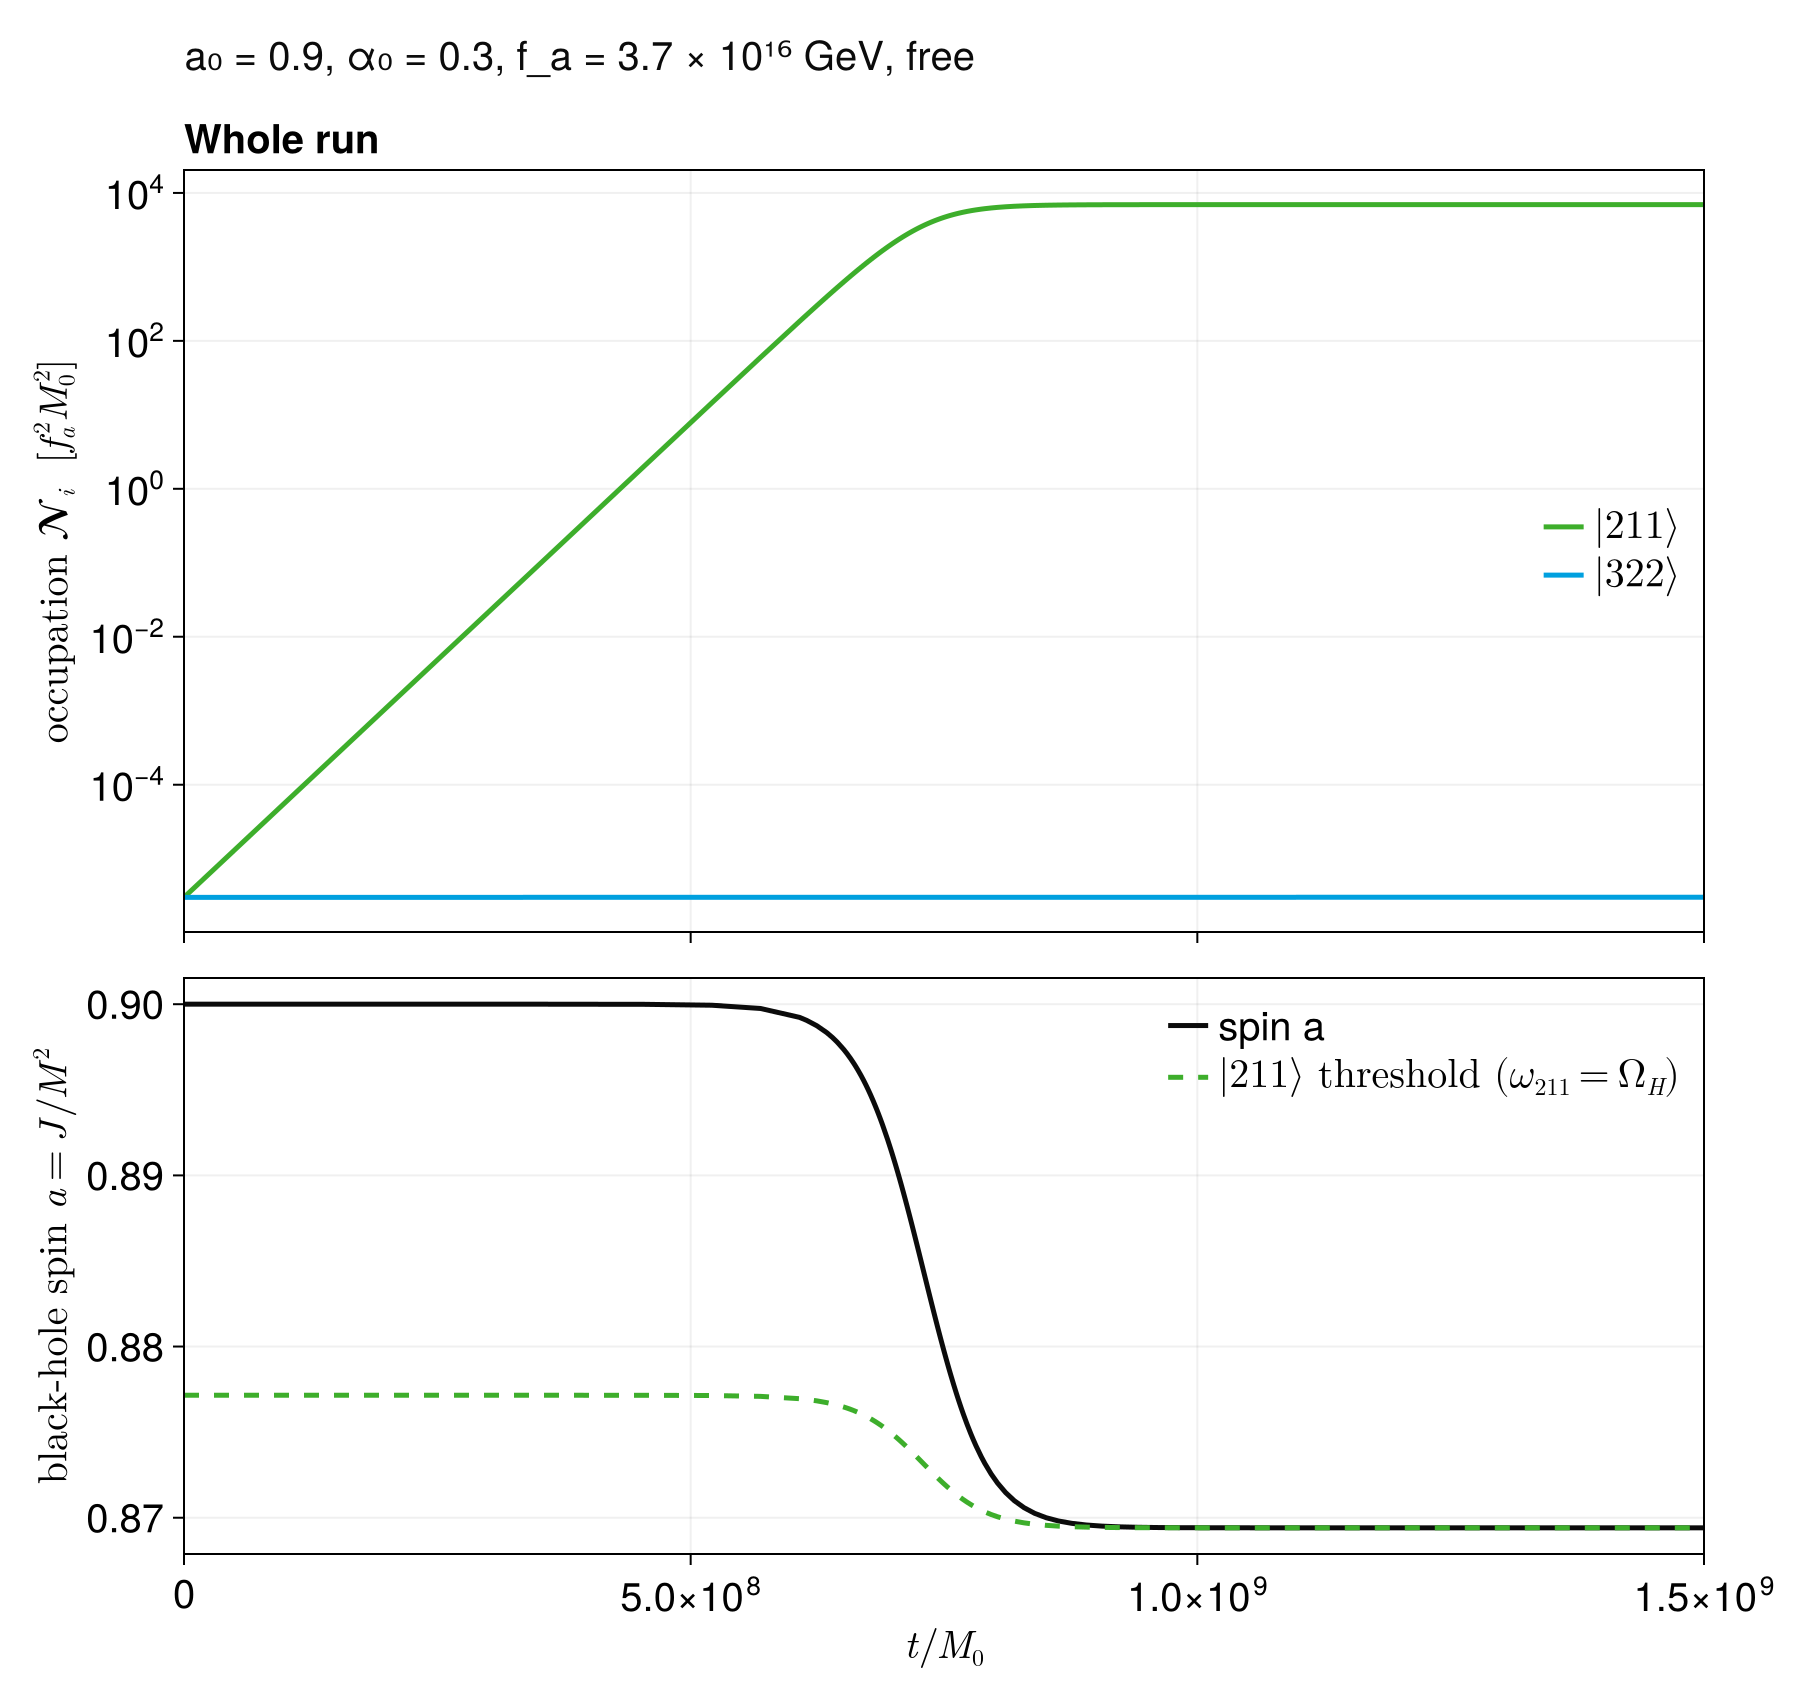
\includegraphics[height=0.8\textheight,width=\textwidth,keepaspectratio]{spindown_free_a0.9_alpha0.3_fa3e-3_compact.png}
    \end{column}
    \begin{column}{0.42\textwidth}
      \small
      Spin locks onto the moving $\ket{211}$ threshold ($\omega_{211} = \Omega_H$).

      \medskip
      \footnotesize
      \begin{tabular}{@{}lccc@{}}
        \toprule
        run & final $a$ & $M/M_0$ & $\mathcal{N}_{211}$ \\
        \midrule
        free & 0.86941 & 0.981478 & 6944 \\
        $5.7\times10^{18}$ GeV & 0.86941 & 0.981478 & 0.2867 \\
        $5.7\times10^{17}$ GeV & 0.86941 & 0.981475 & 28.68 \\
        \bottomrule
      \end{tabular}

      \medskip
      \small
      \begin{itemize}
        \item $\mathcal{N}$ in units of $\fa^2 M_0^2$: ratios $100.01$ and $24219$ match $\kappa$ ratios.
        \item Time-shifted trajectories agree to $\le 3\times10^{-5}$ in $a$.
        \item Lost $J$ / lost $M$ = 3.4 = $m/\omega_{211}$.
      \end{itemize}
    \end{column}
  \end{columns}
\end{frame}

% ---------------------------------------------------------------------------------------------------------------
\begin{frame}{Self-interaction changes the path: $\fa = 3.7\times10^{16}$ GeV, $a_0 = 0.9$}
  \begin{columns}[T]
    \begin{column}{0.62\textwidth}
      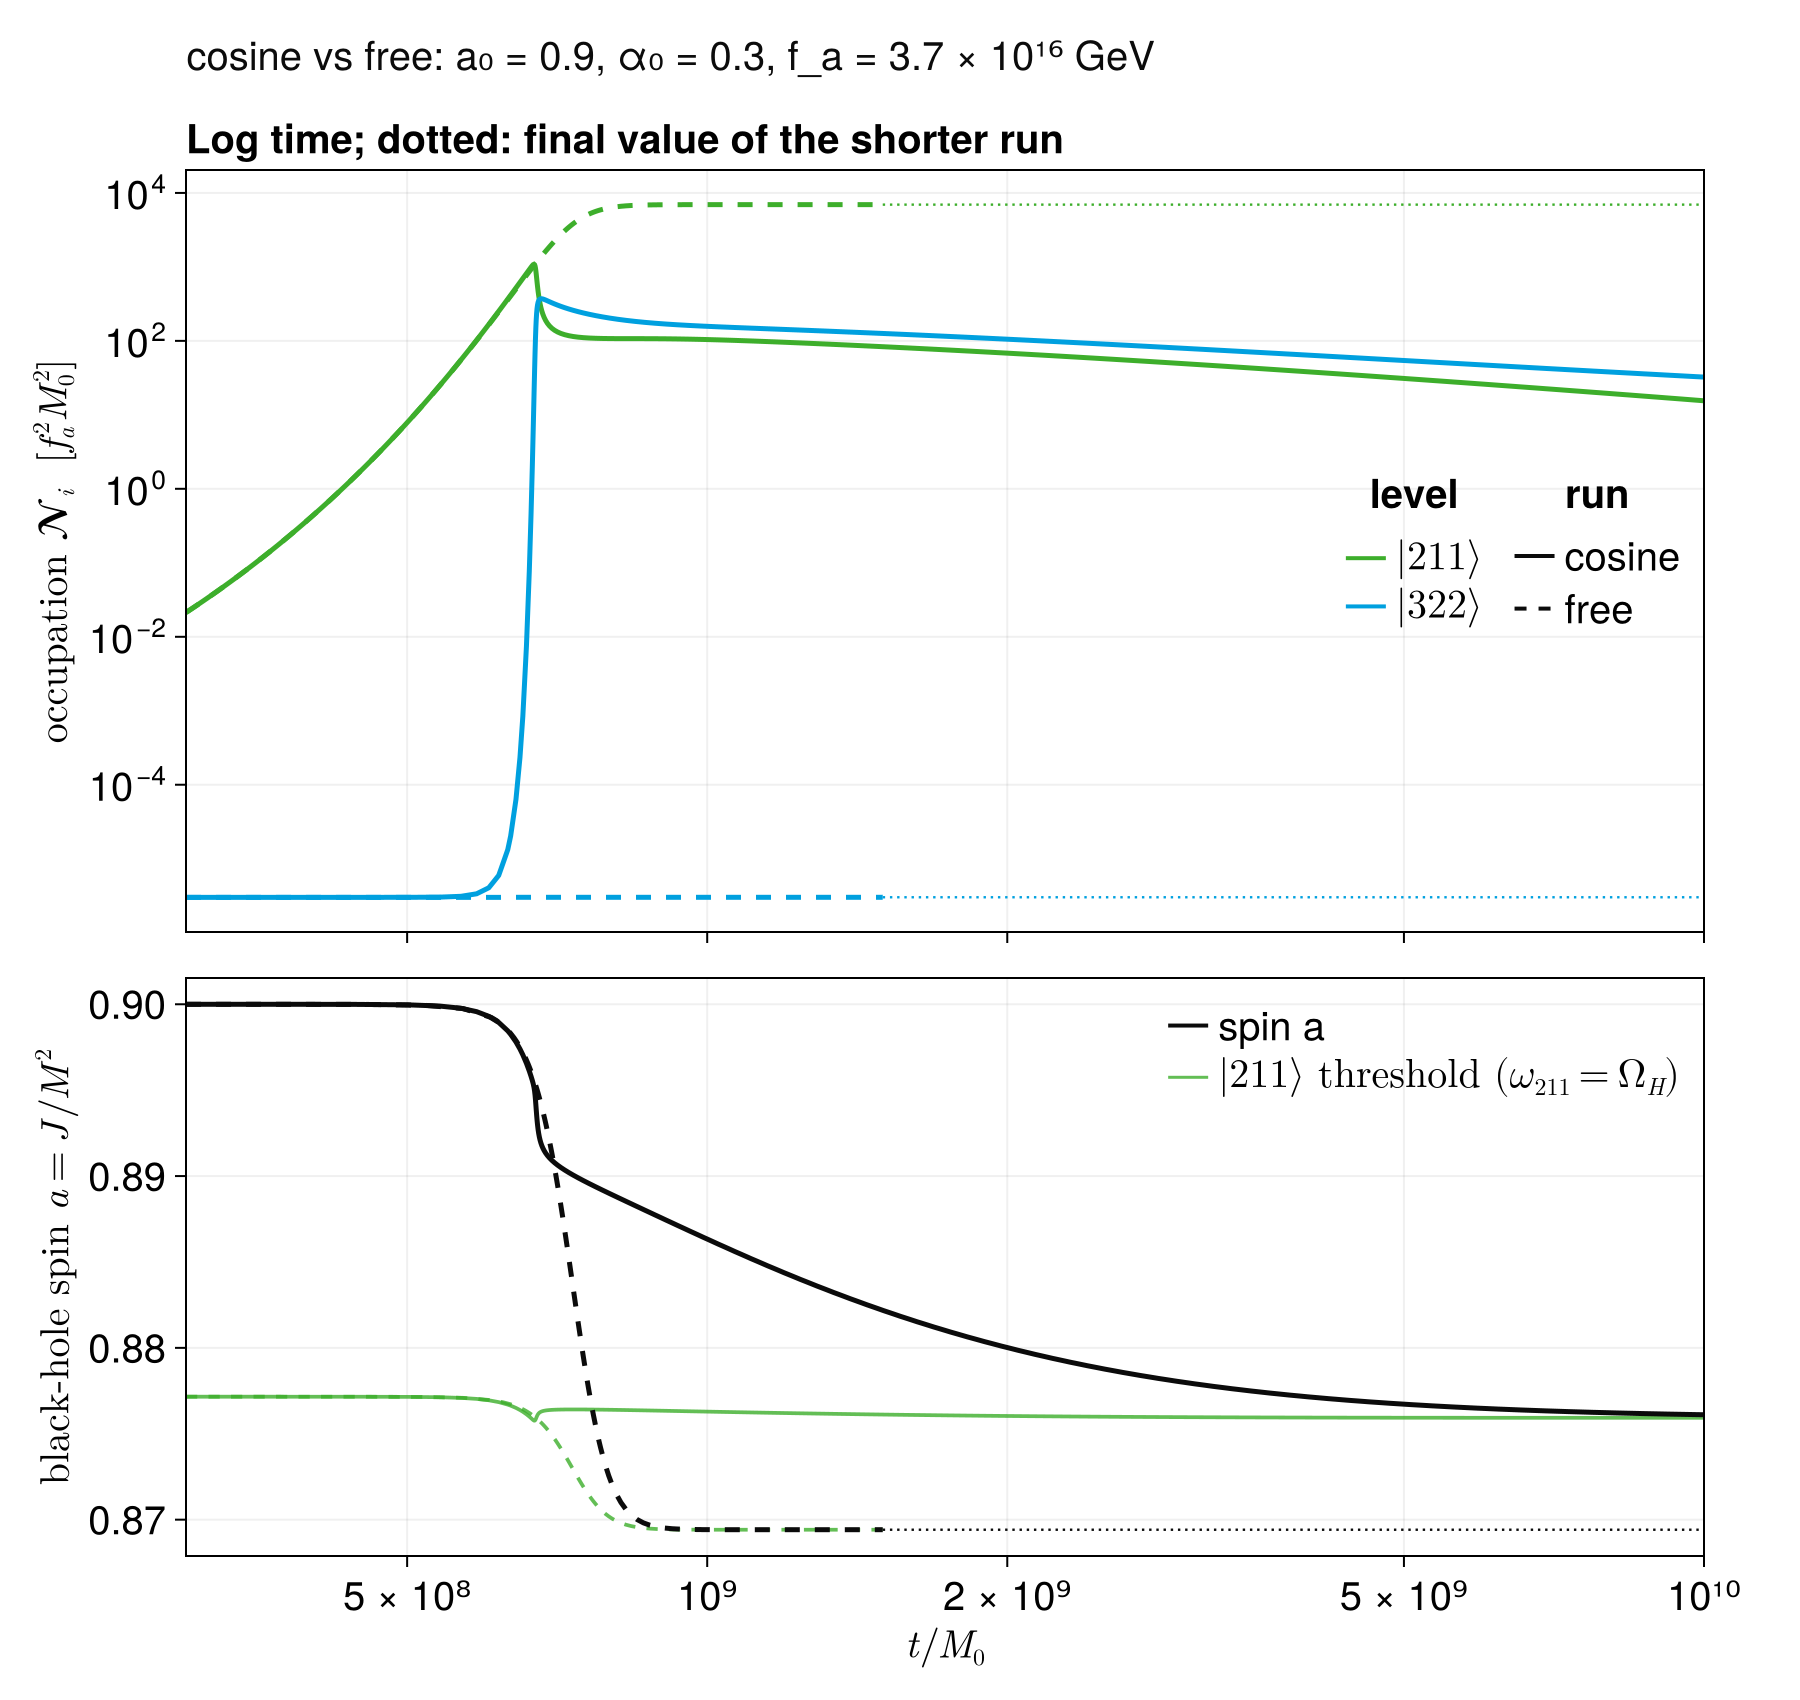
\includegraphics[height=0.8\textheight,width=\textwidth,keepaspectratio]{spindown_overlay_cosine_free_a0.9_alpha0.3_fa3e-3_compact.png}
    \end{column}
    \begin{column}{0.36\textwidth}
      \footnotesize
      \begin{tabular}{@{}lcc@{}}
        \toprule
        & free & cosine \\
        \midrule
        peak $\mathcal{N}_{211}$ & 6944 & 1086 \\
        final $a$ & 0.8694 & 0.8761 \\
        threshold & 0.8694 & 0.8759 \\
        mass lost & 1.85\,\% & 0.30\,\% \\
        $J$ lost [$M_0^2$] & 0.0625 & 0.0291 \\
        $\Delta J/\Delta M$ & 3.4 & 9.8 \\
        \bottomrule
      \end{tabular}

      \medskip
      \small
      \begin{itemize}
        \item $\ket{211}$ collapses at $\mathcal{N}\approx 1086$, $\ket{322}$ jumps by $10^{8}$.
        \item Both end near their own threshold, but the cosine hole gets there losing half the $J$ and $1/6$ of the mass.
        \item Cosine run still approaching threshold at $10^{10} M_0$ ($\approx 23$ d at $40\,\Msun$).
      \end{itemize}
    \end{column}
  \end{columns}
\end{frame}

% ---------------------------------------------------------------------------------------------------------------
\begin{frame}{Why the self-interacting hole spins down more slowly}
  \begin{columns}[T]
    \begin{column}{0.5\textwidth}
      \small
      Spin-down rate $\approx$ (superradiant rate per quantum at this $a$) $\times\ \mathcal{N}_{211}$.
      \begin{itemize}
        \item Free: $\ket{211}$ grows until it holds all the available $J$; the spin falls while $\mathcal{N}_{211}\sim 10^3$--$10^4$.
        \item Cosine: transfer $2\times\ket{211}\to\ket{322}$ caps $\ket{211}$ on a plateau, $\mathcal{N}_{211}\sim 100$
              (superradiant gain = loss to $\ket{322}$).
        \item Plateau $\mathcal{N}$ in $\fa^2$ units is $\fa$-independent; free saturation $\propto (\MPl/\fa)^2$.
              Slow-down factor $\propto (\MPl/\fa)^2$, as in Baryakhtar et al.\ (2011.11646).
        \item Plateau shrinks as $a\to a_c$, so the spin creeps toward threshold.
      \end{itemize}
    \end{column}
    \begin{column}{0.48\textwidth}
      \footnotesize
      Matched spin, after the cosine collapse (finite differences of accepted states):

      \medskip
      \begin{tabular}{@{}cccc@{}}
        \toprule
        $a$ & $\dot a_{\mathrm{free}}/\dot a_{\cos}$ & $\mathcal{N}^{\mathrm{free}}_{211}/\mathcal{N}^{\cos}_{211}$ & $\mathcal{N}^{\cos}_{211}$ \\
        \midrule
        0.889 & 14  & 24  & 108 \\
        0.885 & 25  & 35  & 99 \\
        0.880 & 70  & 68  & 68 \\
        0.878 & 164 & 103 & 49 \\
        \bottomrule
      \end{tabular}

      \medskip
      Rate tracks $\mathcal{N}_{211}$ to within $\approx 1.6\times$.
      Residual not separated: extra spin-down from $\ket{322}$ and the $m=0$ channel at high $a$;
      different thresholds (different mass loss) near $a_c$.
    \end{column}
  \end{columns}
\end{frame}

% ---------------------------------------------------------------------------------------------------------------
\begin{frame}{Even QCD-sized $\fa$ is not free at late times ($5.7\times10^{17}$ GeV, $4\,\Msun$)}
  \begin{columns}[T]
    \begin{column}{0.6\textwidth}
      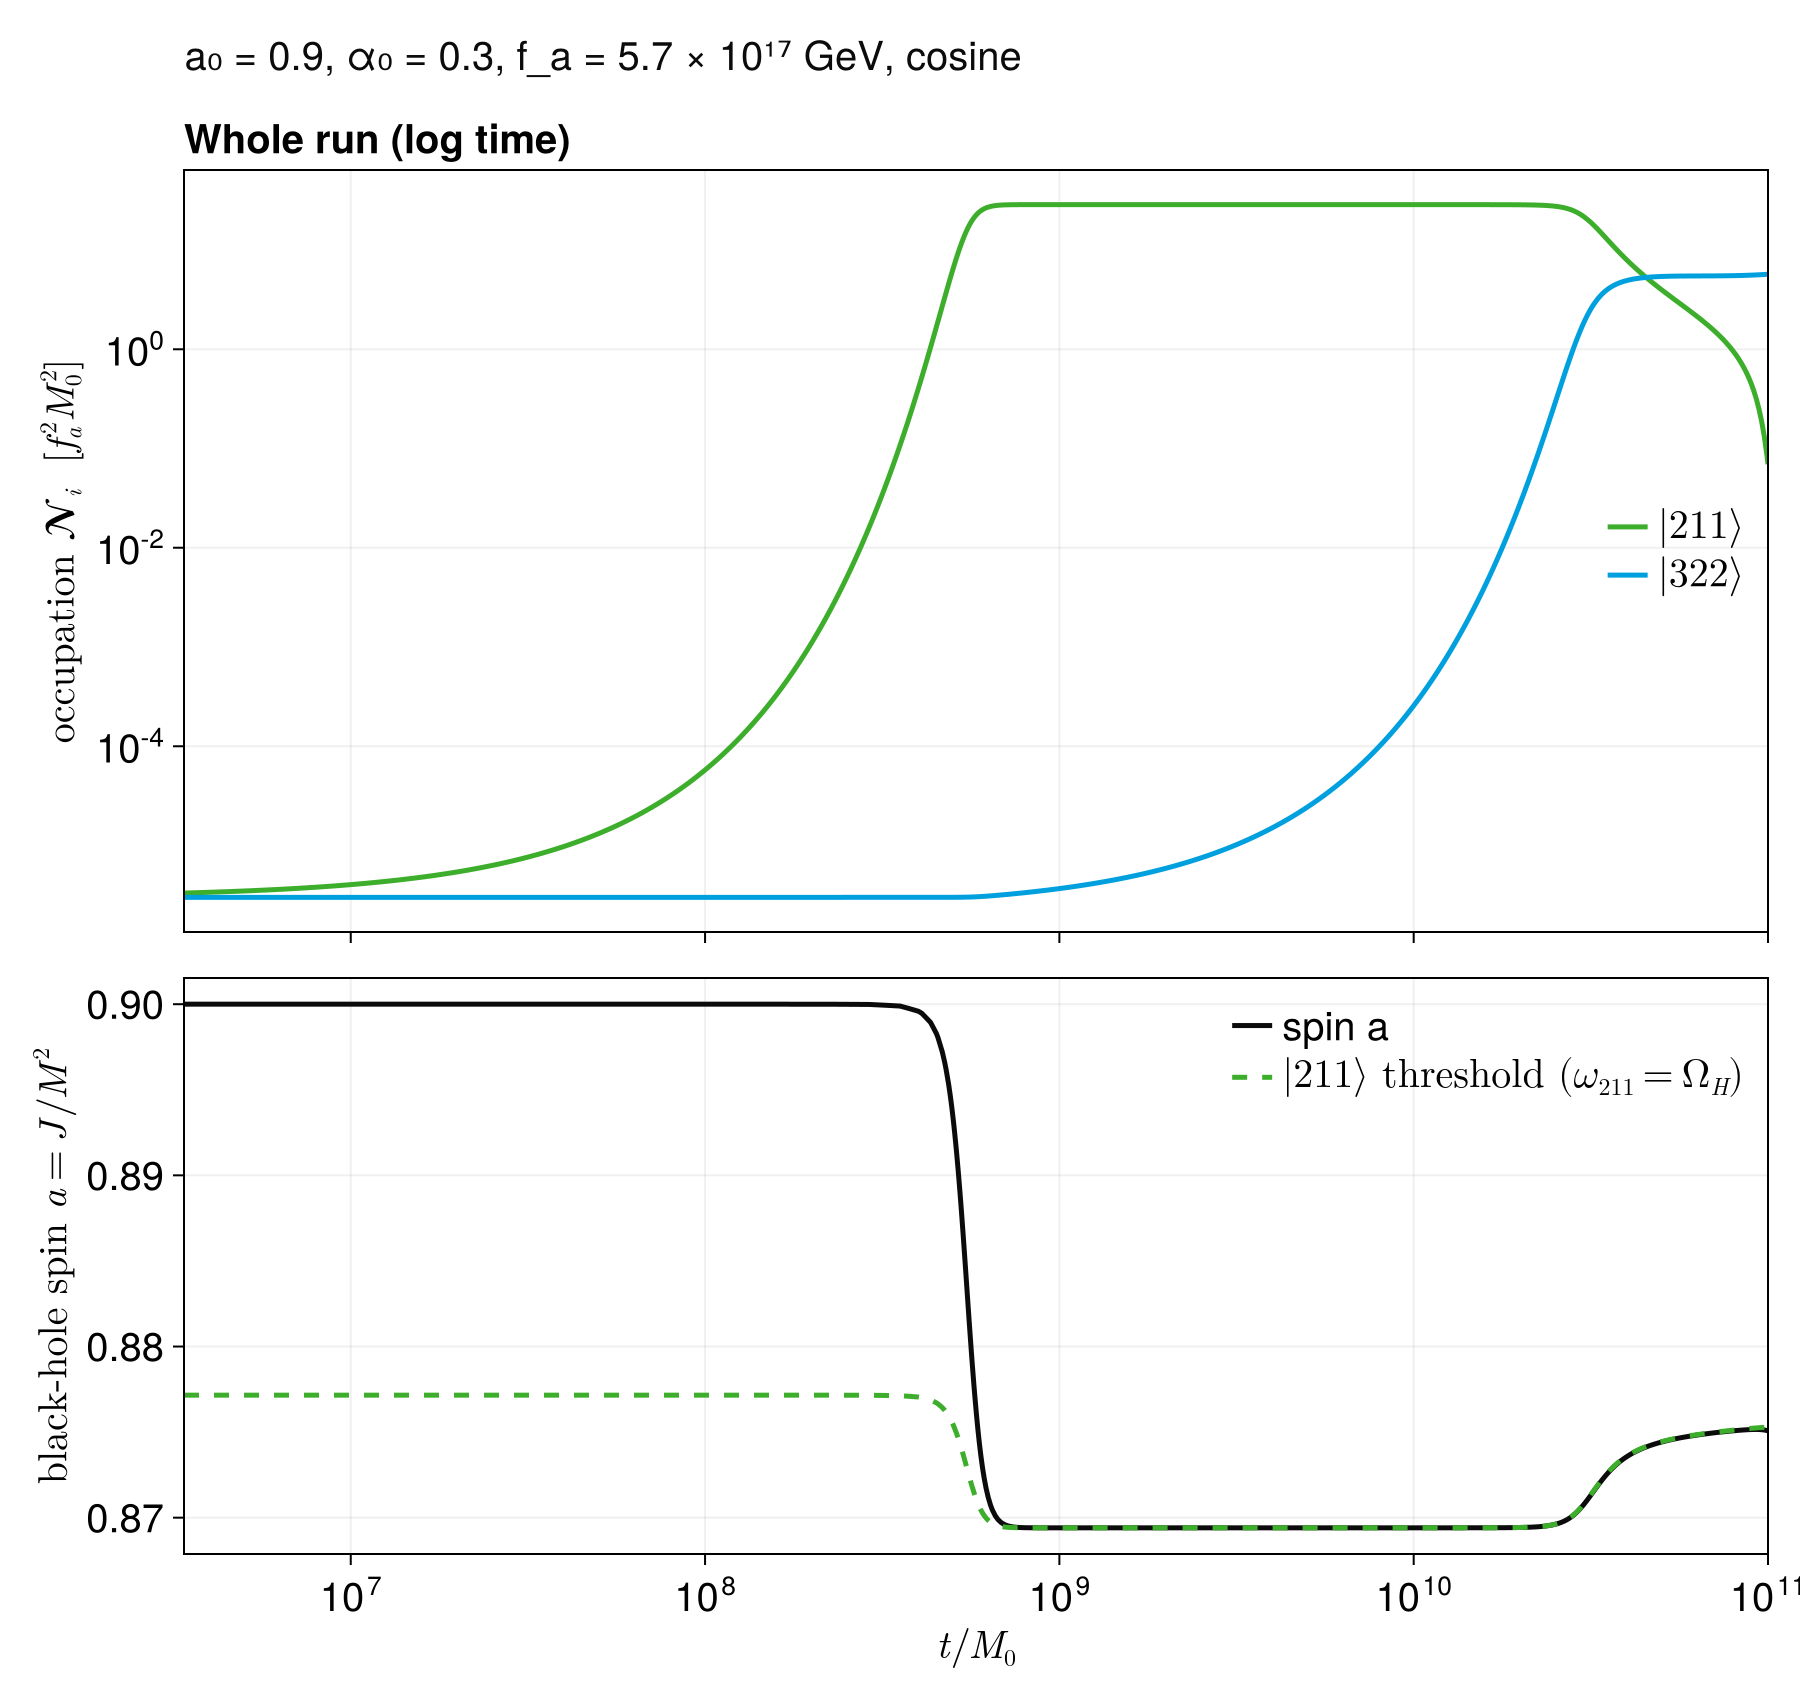
\includegraphics[height=0.8\textheight,width=\textwidth,keepaspectratio]{spindown_a0.9_alpha0.3_fa0.0466873_t1e11_restart_compact.png}
    \end{column}
    \begin{column}{0.38\textwidth}
      \small
      Restart of the saturated run to $10^{11} M_0$ ($\approx 23$ d at $4\,\Msun$).
      \begin{itemize}
        \item $\ket{322}$ grows $200\times$ faster than free; excess rate $\propto \mathcal{N}_{211}^2$
              (checked across the two QCD runs: ratio $10^4$ for $\kappa$ ratio $10^2$).
        \item $\ket{322}$ stalls at $\mathcal{N}\approx 5.7$ (expected 50--100).
        \item $\ket{211}$ is reabsorbed ($\times 1/400$); hole \emph{regains} mass, $M/M_0$: $0.9815\to0.9955$.
        \item Spin rises $0.8694\to0.8751$, tracking the threshold from just below.
      \end{itemize}
      \footnotesize
      At $5.7\times10^{18}$ GeV the same excess is $2\,\%$ of the free rate.
    \end{column}
  \end{columns}
\end{frame}

% ---------------------------------------------------------------------------------------------------------------
\begin{frame}{Mechanism: the $m=0$ component $X$ is absorbed by the hole}
  \begin{columns}[T]
    \begin{column}{0.5\textwidth}
      \small
      Component $\mathbf{q}=(q_1,q_2)$ of the field: phase $q_1\xi_{211}+q_2\xi_{322}$ ($\xi_i$ = phase of mode $i$, as in
      multiphase.tex), frequency $q_1\omega_{211}+q_2\omega_{322}$, $m = q_1 + 2q_2$. Call $X \equiv (2,-1)$:
      \[ \omega_X = 2\omega_{211}-\omega_{322} \approx 0.289 < \mu M, \qquad m_X = 0. \]
      \centering
      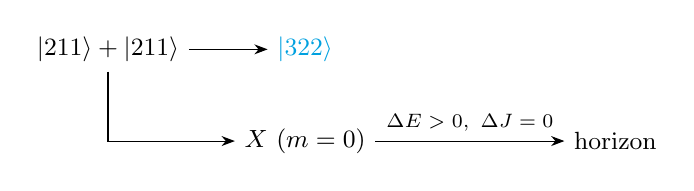
\begin{tikzpicture}[node distance=6mm and 10mm, every node/.style={font=\small}]
        \node (a) {$\ket{211}+\ket{211}$};
        \node[right=of a] (b) {$\textcolor{blue322}{\ket{322}}$};
        \node[below=of b] (c) {$X$ ($m=0$)};
        \node[right=24mm of c] (h) {horizon};
        \draw[-{Stealth}] (a) -- (b);
        \draw[-{Stealth}] (a) |- (c);
        \draw[-{Stealth}] (c) -- node[above,font=\scriptsize]{$\Delta E>0,\ \Delta J=0$} (h);
      \end{tikzpicture}
      \raggedright
      \begin{enumerate}
        \item $X$ cannot escape to infinity; at $m=0$ it is never superradiant.
        \item Energy without $J$ lowers $a=J/M^2$ below the $\ket{211}$ threshold.
        \item $\ket{211}$ is then absorbed, raising $a$; the mass gain raises $\alpha$ and the threshold.
      \end{enumerate}
    \end{column}
    \begin{column}{0.48\textwidth}
      \footnotesize
      Horizon flux by channel at $t = 2.9\times10^{10}$ (rebuilt solution):

      \medskip
      \begin{tabular}{@{}lccc@{}}
        \toprule
        channel & $m$ & $F_E^{\mathrm{H}}$ & $\dot a$ part \\
        \midrule
        $(1,0)=\ket{211}$ & 1 & $+2.3\times10^{-10}$ & $+8.6\times10^{-13}$ \\
        $(0,1)=\ket{322}$ & 2 & $-1.0\times10^{-12}$ & $-1.1\times10^{-14}$ \\
        $(2,-1)=X$ & 0 & $+1.3\times10^{-10}$ & $-5.2\times10^{-13}$ \\
        \midrule
        net & & & $+3.3\times10^{-13}$ \\
        \bottomrule
      \end{tabular}

      \medskip
      \begin{itemize}
        \item Every channel has the sign of $\omega_c(\omega_c - m_c\Omega_H)$; channel sum = total flux to $5\times10^{-26}$.
        \item Threshold slope $0.415$ per unit $M/M_0$ (free run) predicts final threshold $0.87521$; recorded $0.87528$.
        \item Not checked: is $X$ resolved ($l=0$ only)?
      \end{itemize}
    \end{column}
  \end{columns}
\end{frame}

% ---------------------------------------------------------------------------------------------------------------
\begin{frame}{Competing regime (preliminary): $a_0 = 0.99$, $\fa = 1.2\times10^{17}$ GeV}
  \begin{columns}[T]
    \begin{column}{0.6\textwidth}
      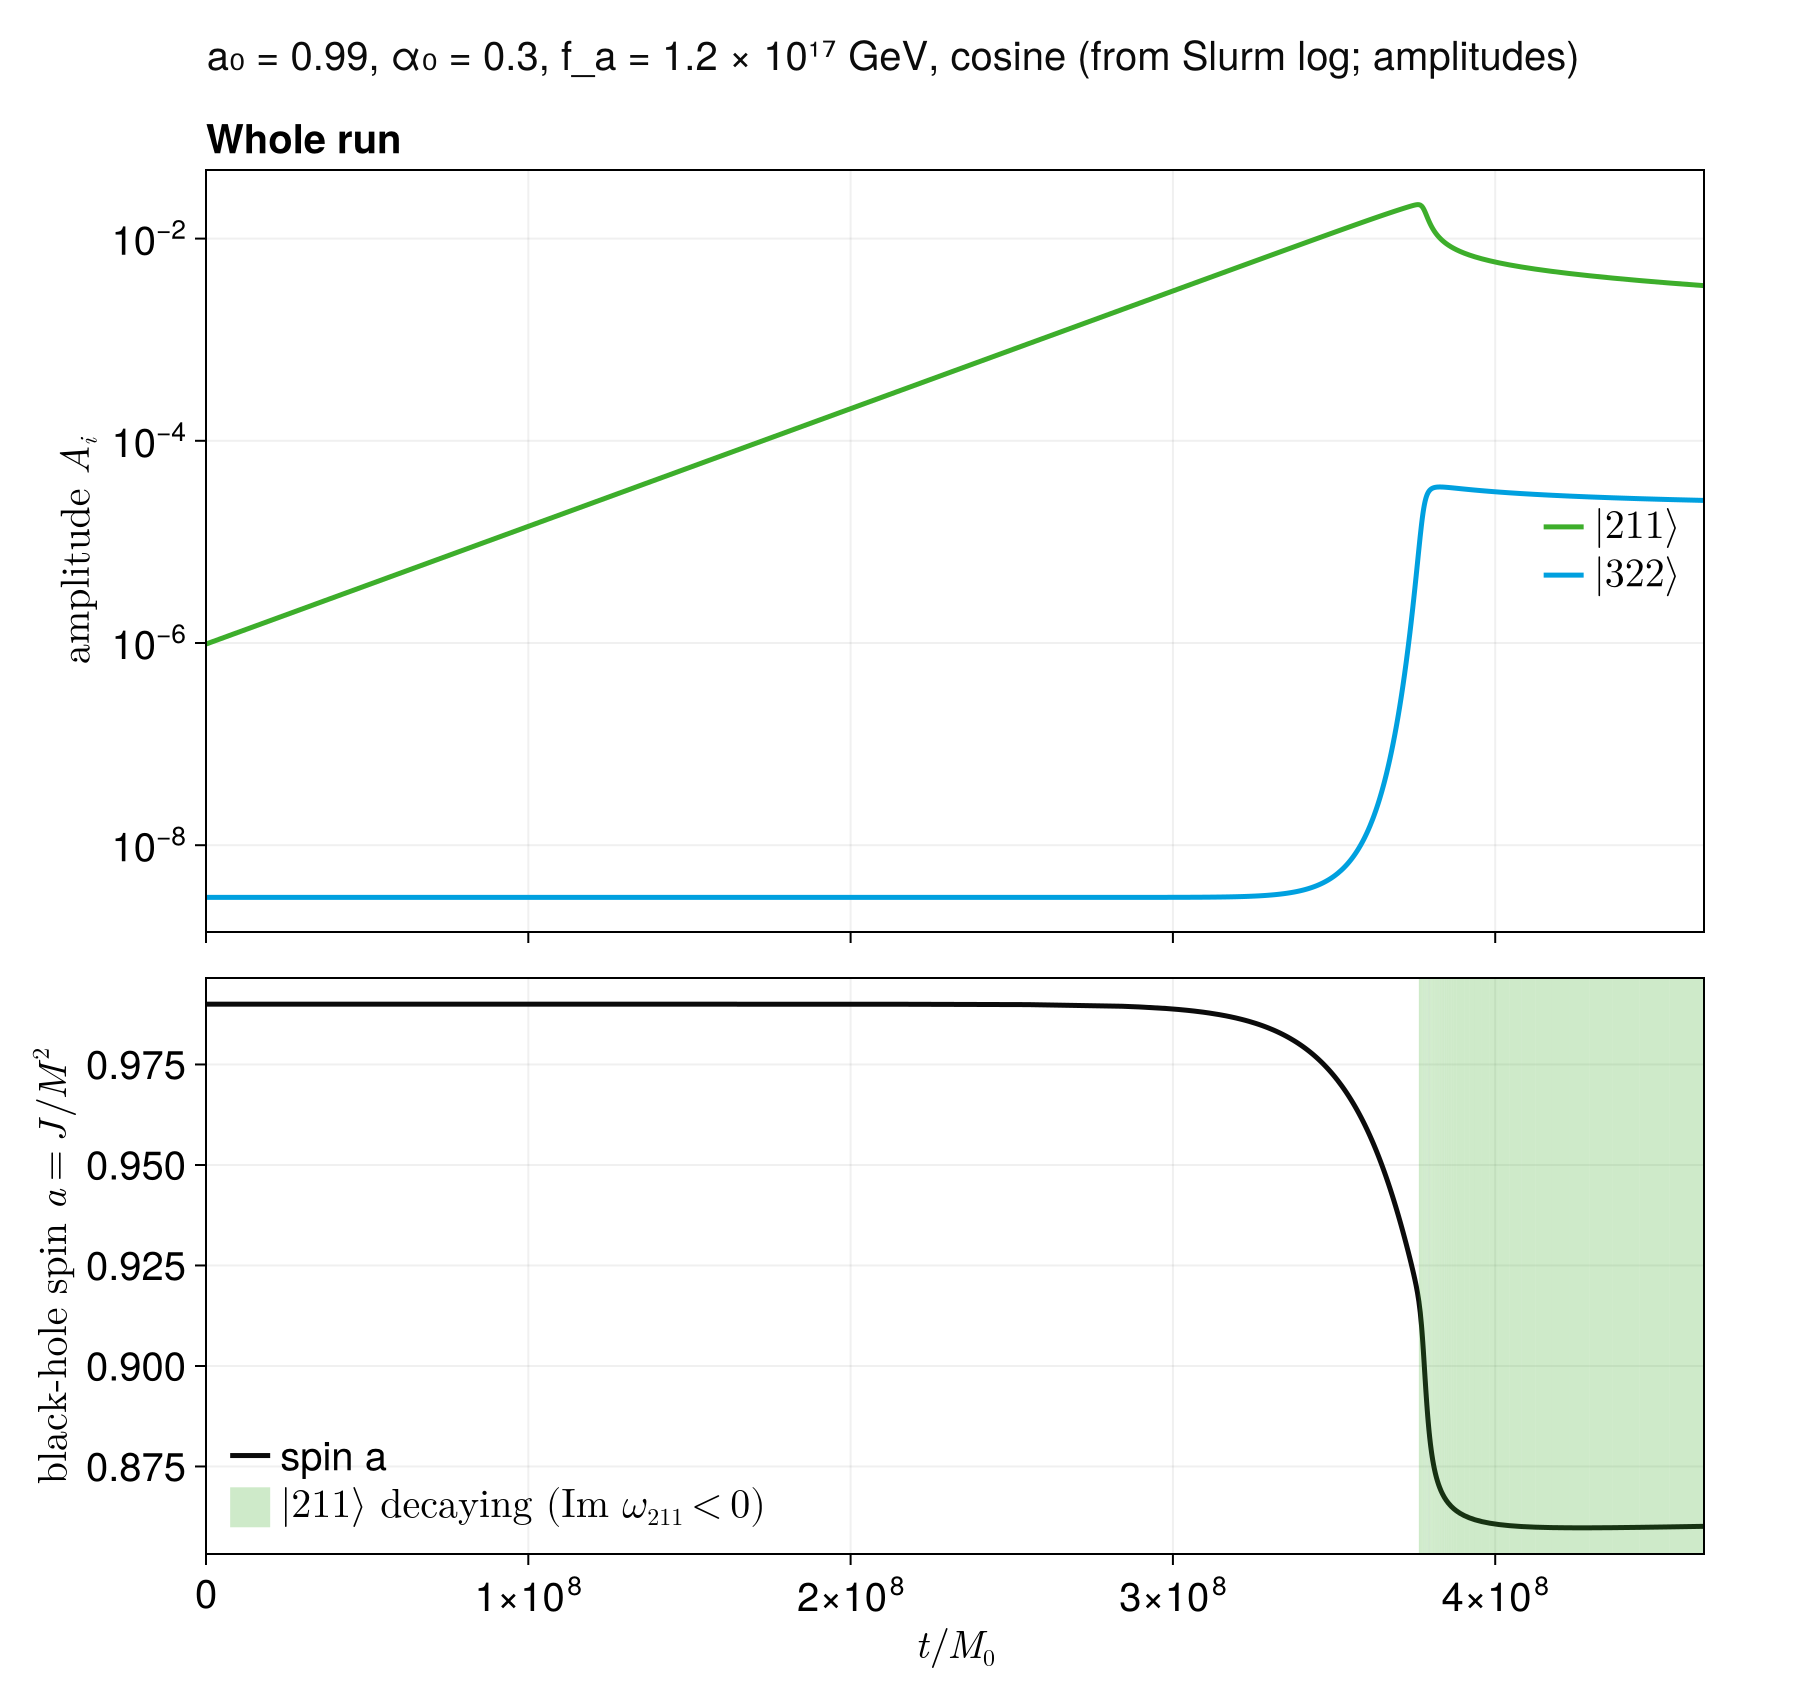
\includegraphics[height=0.8\textheight,width=\textwidth,keepaspectratio]{spindown_a0.99_alpha0.3_fa1e-2_partial_compact.png}
    \end{column}
    \begin{column}{0.38\textwidth}
      \small
      \begin{itemize}
        \item Peak mass loss 4.5\,\% ($M/M_0 = 0.955$ at $3.77\times10^8$).
        \item $\ket{322}$ grows at $7\times10^{-7}$, $4\times10^5\times$ its linear rate, while $\ket{211}$ peaks.
        \item Spin crashes $0.918\to0.869$ in $\approx 7\times10^6 M_0$ and overshoots to $0.860$, below the $\ket{211}$ threshold.
        \item Both levels then absorbed; mass recovers to $0.980$.
      \end{itemize}
      \footnotesize
      Caveats: job timed out at $4.8\times10^8$ (no CSV; plot from log, amplitudes not occupations);
      mesh built at $a=0.99$ used at $0.86$; flux-sign test not run.
    \end{column}
  \end{columns}
\end{frame}

% ---------------------------------------------------------------------------------------------------------------
\begin{frame}{Quasi-static plateau spin-down vs Baryakhtar et al.\ Fig.~9}
  \begin{columns}[T]
    \begin{column}{0.6\textwidth}
      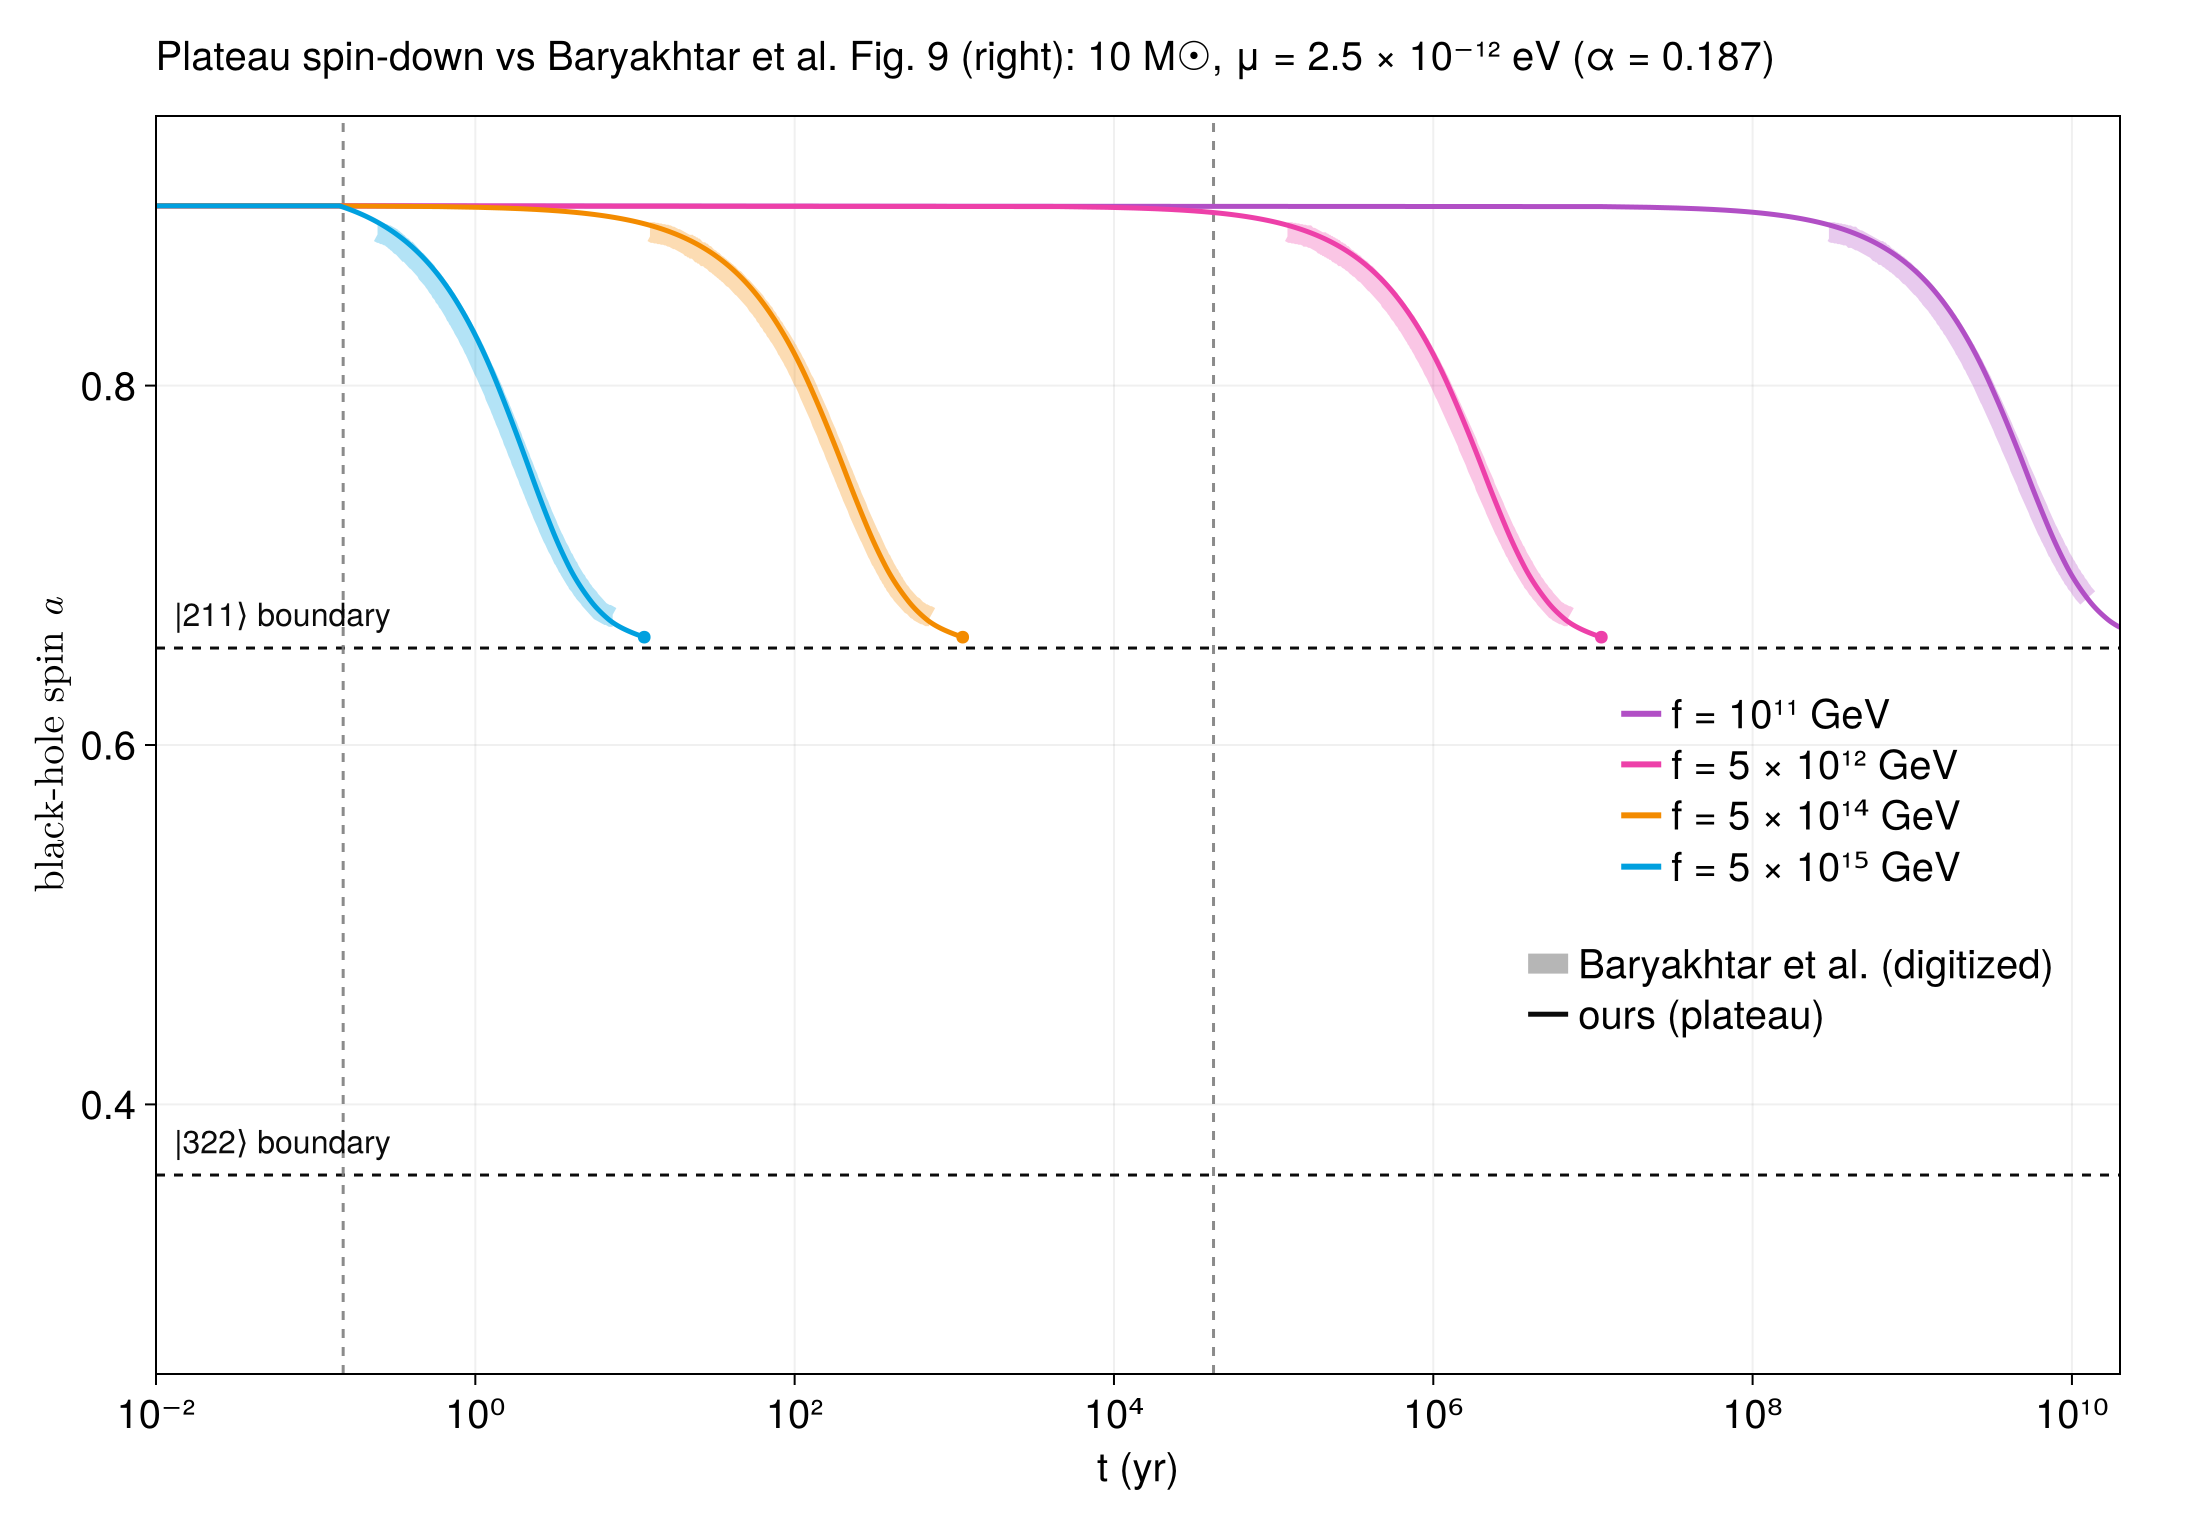
\includegraphics[width=\textwidth]{baryakhtar_fig9_comparison.png}
    \end{column}
    \begin{column}{0.38\textwidth}
      \footnotesize
      $10\,\Msun$, $m_a = 2.5\times10^{-12}$ eV ($\alpha = 0.187$). For small $\fa$ the hole moves $(\MPl/\fa)^2$ times
      slower than the plateau relaxes, so track the plateau:
      \[ \dot a = \kappa\,\big(F_J^{\mathrm{H}} - 2a F_E^{\mathrm{H}}\big) \equiv -\kappa\, D(a) \]
      ($M$, $\alpha$ fixed; clock starts after free growth to the plateau, $\approx 0.13$ yr).
      \begin{itemize}
        \item Against their digitized curves: our $t(a)$ is $6$--$9\,\%$ longer at $a = 0.78$, $2\,\%$ at $a = 0.70$,
              for every $f$.
        \item Near threshold ($a_c = 0.654$): $\mathcal{N}_{211}\propto (a-a_c)^{1/2}$, $D\propto(a-a_c)^{3/2}$, as in their
              equilibrium formulas.
        \item Free spin-down times: $0.149$ yr ($\ket{211}$), $4.2\times10^4$ yr ($\ket{322}$, at $a=0.654$) vs their
              $0.146$, $5.0\times10^4$ (dashed lines).
      \end{itemize}
      Not yet: $f \ge 5\times10^{16}$ GeV and the $\ket{322}$ stage (need full evolution at $\alpha=0.187$); mesh convergence.
    \end{column}
  \end{columns}
\end{frame}

% ---------------------------------------------------------------------------------------------------------------
\begin{frame}{Summary, open questions, next steps}
  \begin{columns}[T]
    \begin{column}{0.5\textwidth}
      \small
      \textbf{Summary}
      \begin{itemize}
        \item Coupled cloud + hole evolution runs end to end; large $\fa$ reproduces free spin-down.
        \item Self-interaction caps $\ket{211}$: slower spin-down, $6\times$ less mass loss, larger $\Delta J/\Delta M$.
        \item The $m=0$ partner of $2\times\ket{211}\to\ket{322}$ feeds energy (no $J$) back into the hole;
              at late times this reabsorbs $\ket{211}$ even at QCD-sized $\fa$.
        \item Plateau spin-down matches Baryakhtar et al.\ Fig.~9 to $\lesssim 10\,\%$ in time.
      \end{itemize}
    \end{column}
    \begin{column}{0.48\textwidth}
      \small
      \textbf{Open / to discuss}
      \begin{itemize}
        \item GW annihilation of $\ket{211}$: does it act on the $10^{10}$--$10^{11} M_0$ times of the $m=0$ effect?
        \item Is the $(2,-1)$ channel resolved with $l=0$ only?
        \item Levels with $m\ge3$ omitted.
      \end{itemize}
      \textbf{Next}
      \begin{itemize}
        \item Free + cosine pair at $\alpha=0.187$ (direct test of the plateau method).
        \item Restart $a_0 = 0.99$ runs; containment check at low spin.
        \item Mesh-convergence check along one trajectory.
      \end{itemize}
    \end{column}
  \end{columns}
\end{frame}

\end{document}
